\chapter{gfortranのインストール}
gfortranはフリーのコンパイラであるから,
自分のもっているノートPCや家にあるPCにインストールしておくのがよい.
その手順を以下に記す.

\begin{enumerate}
\item https://sourceforge.net/projects/mingw-w64/ にアクセスし, mingw-w64-install.exeをダウンロードする.
\item ダウンロードしたmingw-w64-install.exeを実行する.
\item 図\ref{fig_install}(a)で[Next]を押す.
\item 図\ref{fig_install}(b)でVersionは5.2.0以降, Architectureは64bitマシンの場合はx86\_64を選択する. それ以外の項目はデフォルトでよい.
\item 図\ref{fig_install}(c)でインストール先を聞かれるが, デフォルトでよい.
\item 図\ref{fig_install}(d)のようにインストールが始まるのでしばらく待つ.
\item 図\ref{fig_install}(e)で[Next]を押す.
\item 図\ref{fig_install}(f)の画面が出たらインストールは終了である.
\item インストールしたgfortranをコマンドプロンプトから実行するにはgfortranをインストールしたディレクトリにパスを通しておく必要がある.
\textcolor{red}{環境変数の設定を失敗するとシステムが正常に動作しなくなる可能性がある. 自己責任で慎重におこなうこと. }

[コントロールパネル]$\to$[システム]$\to$[システムの詳細設定]$\to$[環境変数]を開く.
\item システム環境変数中のPathを選択し, [編集]を押す.
\item 変数値の末尾にセミコロン(;)を挿入し, 続けて各自がgfortranをインストールしたディレクトリを追加する.
アドレスバーをコピーし, そのまま貼り付けるのがよい. 次はその例である.

C:Y\llap{=}Program FilesY\llap{=}mingw-w64Y\llap{=}x86\_64-6.1.0-posix-seh-rt\_v5-rev0Y\llap{=}mingw64Y\llap{=}bin

\item コマンドプロンプトを立ち上げ, gfortranとタイプする. 画面に no input files と表示されれば, 正しくパスが通っている.
\end{enumerate}

\begin{figure}[ht]
\centering
\subfloat[]{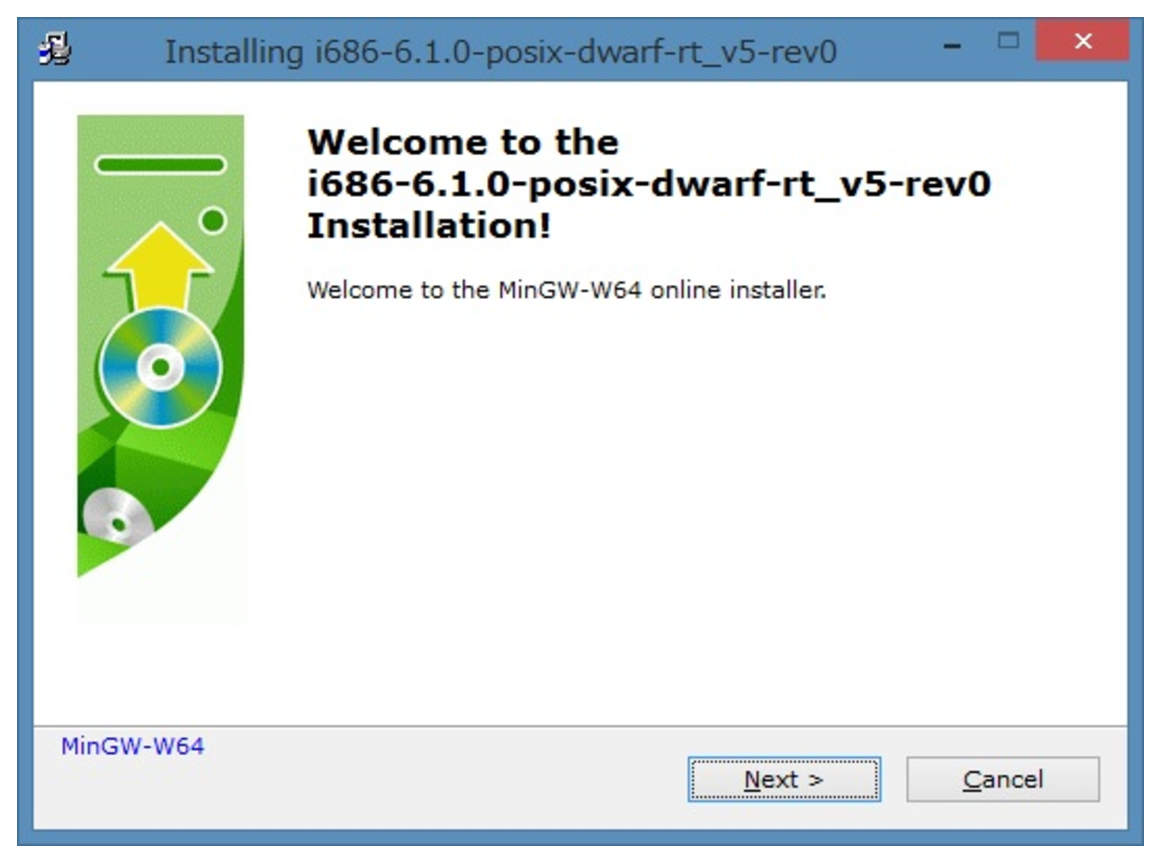
\includegraphics[width=0.45\linewidth]{appendix/install/1/install1.eps}} \hspace{5mm}
\subfloat[]{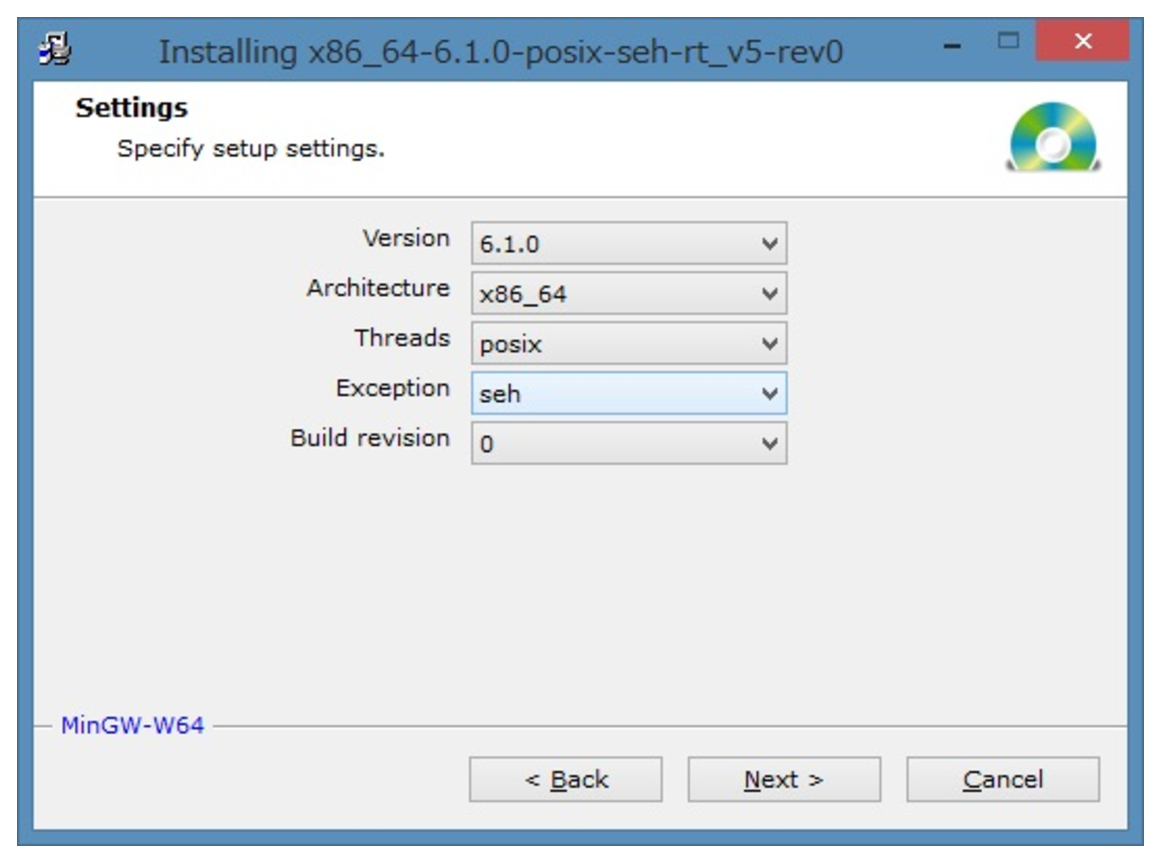
\includegraphics[width=0.45\linewidth]{appendix/install/1/install2.eps}}\\
\subfloat[]{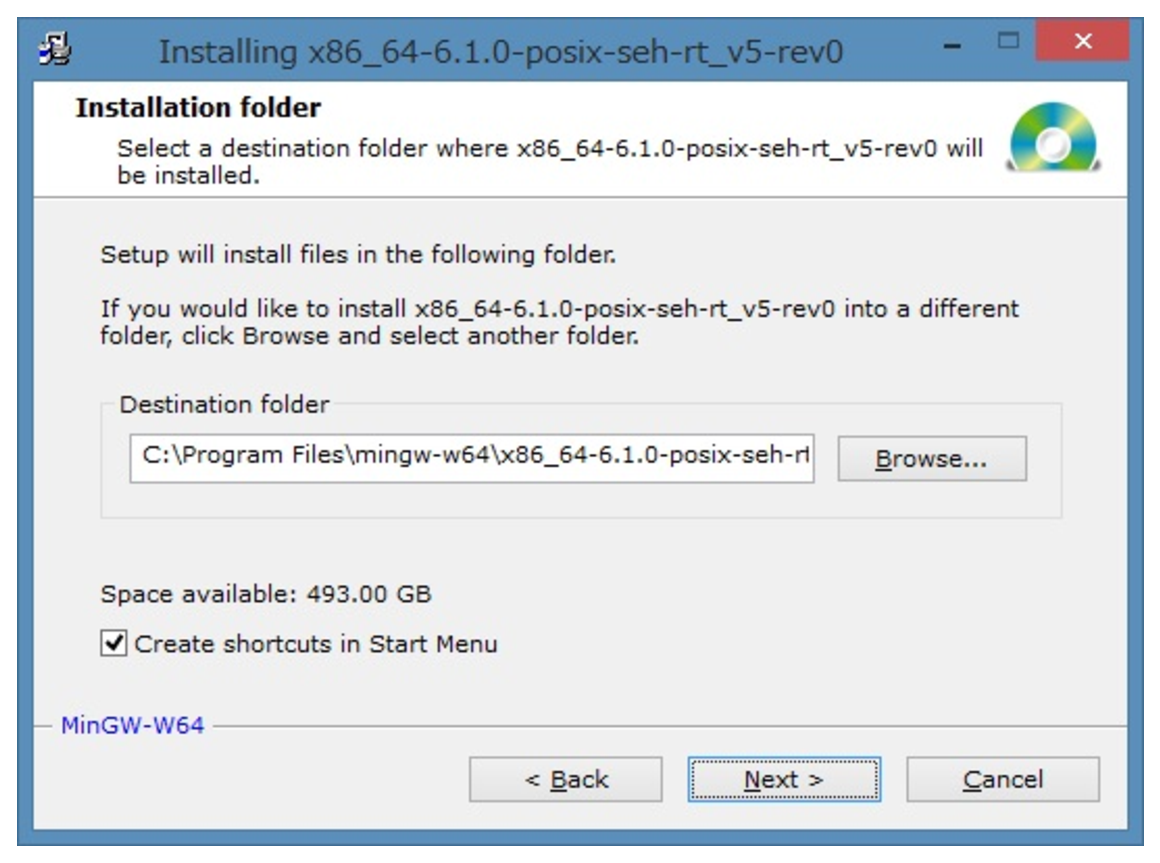
\includegraphics[width=0.45\linewidth]{appendix/install/1/install3.eps}} \hspace{5mm}
\subfloat[]{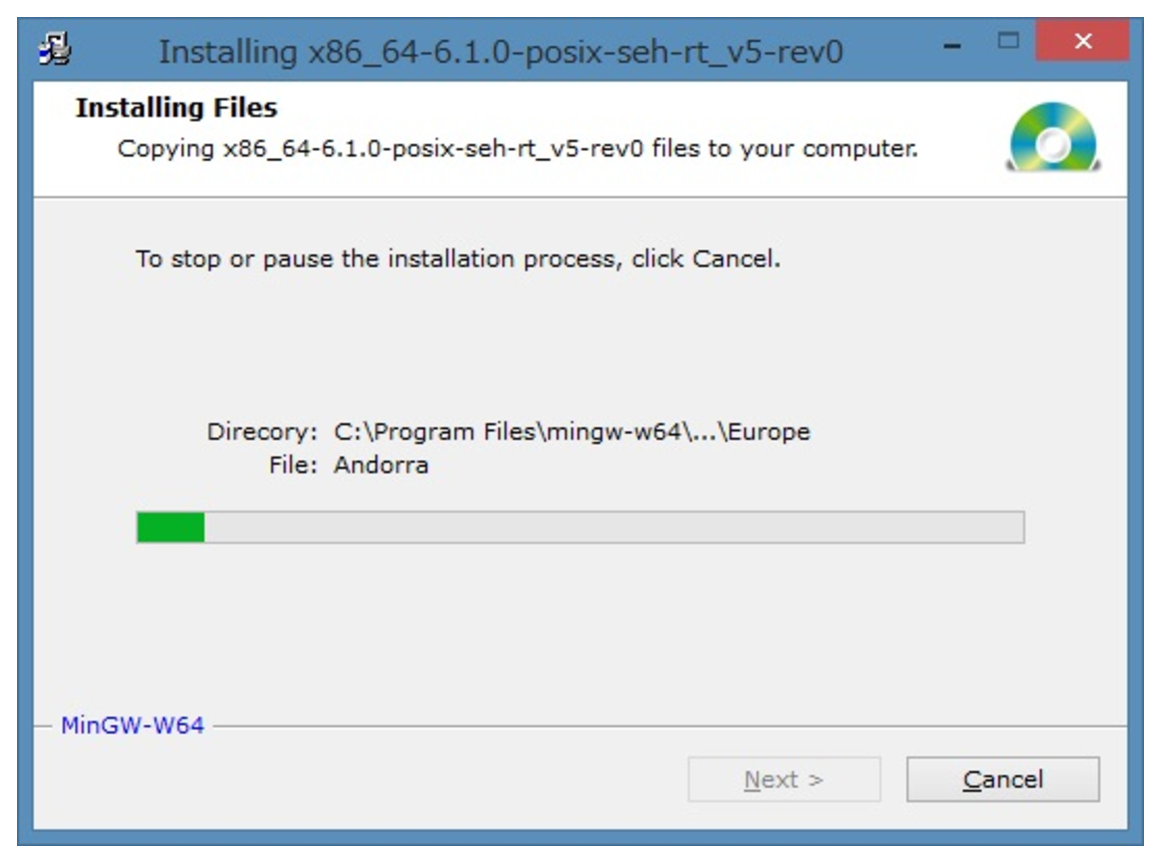
\includegraphics[width=0.45\linewidth]{appendix/install/1/install4.eps}}\\
\subfloat[]{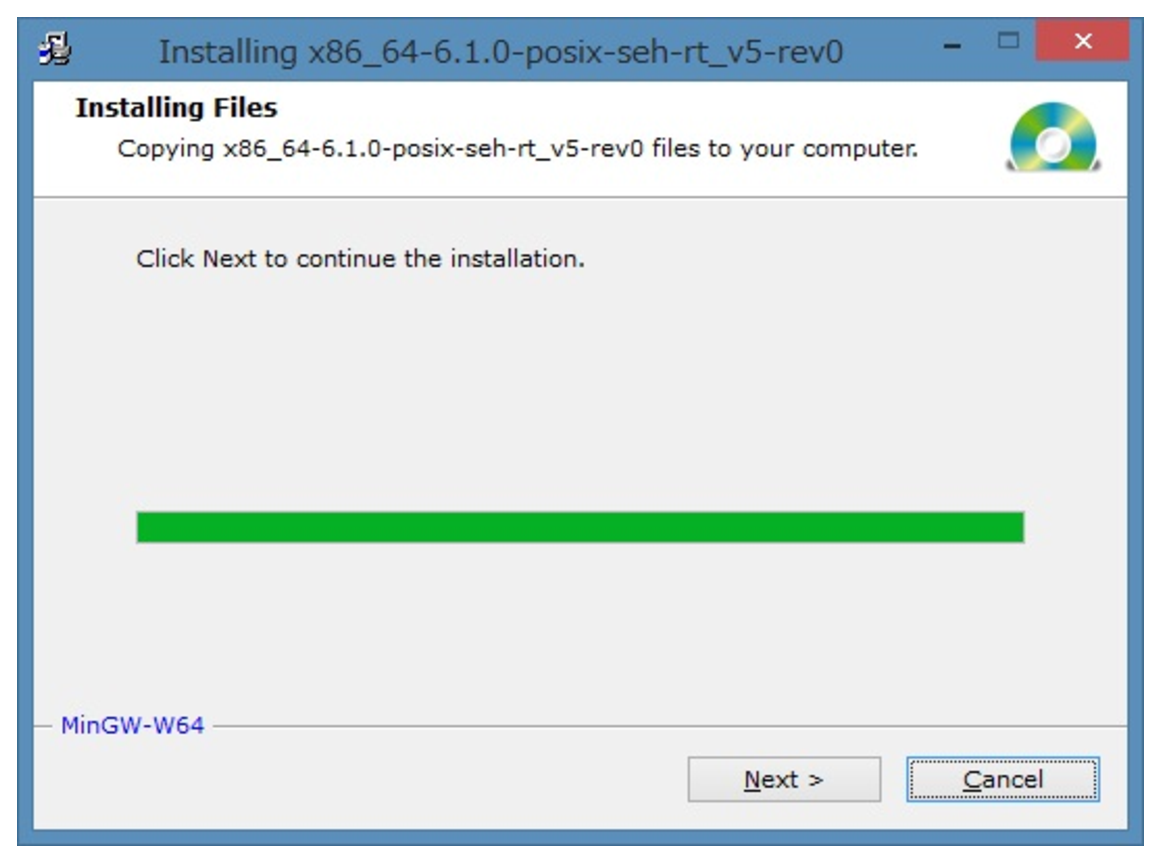
\includegraphics[width=0.45\linewidth]{appendix/install/1/install5.eps}} \hspace{5mm}
\subfloat[]{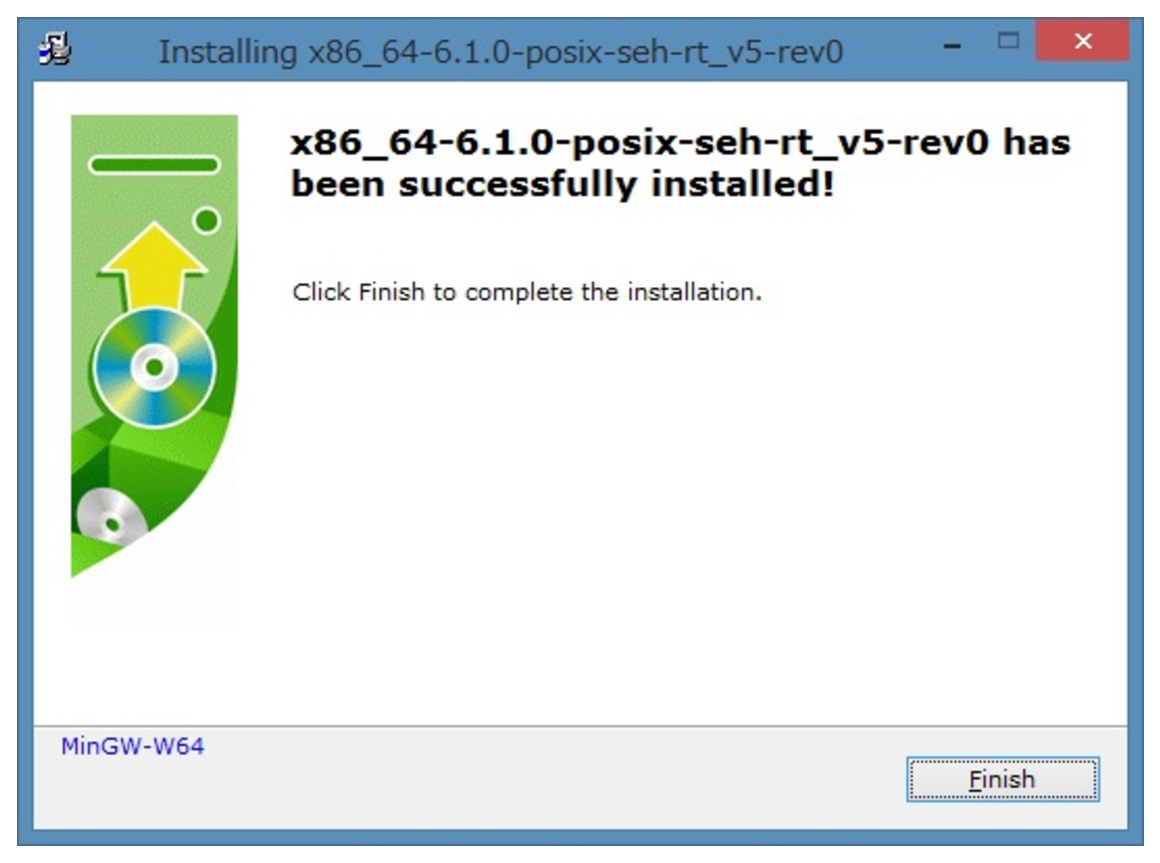
\includegraphics[width=0.45\linewidth]{appendix/install/1/install6.eps}}\\
\caption{gfotranのインストール.  }
\label{fig_install}
\end{figure}
